% Options for packages loaded elsewhere
\PassOptionsToPackage{unicode}{hyperref}
\PassOptionsToPackage{hyphens}{url}
%
\documentclass[
]{article}
\usepackage{amsmath,amssymb}
\usepackage{lmodern}
\usepackage{ifxetex,ifluatex}
\ifnum 0\ifxetex 1\fi\ifluatex 1\fi=0 % if pdftex
  \usepackage[T1]{fontenc}
  \usepackage[utf8]{inputenc}
  \usepackage{textcomp} % provide euro and other symbols
\else % if luatex or xetex
  \usepackage{unicode-math}
  \defaultfontfeatures{Scale=MatchLowercase}
  \defaultfontfeatures[\rmfamily]{Ligatures=TeX,Scale=1}
\fi
% Use upquote if available, for straight quotes in verbatim environments
\IfFileExists{upquote.sty}{\usepackage{upquote}}{}
\IfFileExists{microtype.sty}{% use microtype if available
  \usepackage[]{microtype}
  \UseMicrotypeSet[protrusion]{basicmath} % disable protrusion for tt fonts
}{}
\makeatletter
\@ifundefined{KOMAClassName}{% if non-KOMA class
  \IfFileExists{parskip.sty}{%
    \usepackage{parskip}
  }{% else
    \setlength{\parindent}{0pt}
    \setlength{\parskip}{6pt plus 2pt minus 1pt}}
}{% if KOMA class
  \KOMAoptions{parskip=half}}
\makeatother
\usepackage{xcolor}
\IfFileExists{xurl.sty}{\usepackage{xurl}}{} % add URL line breaks if available
\IfFileExists{bookmark.sty}{\usepackage{bookmark}}{\usepackage{hyperref}}
\hypersetup{
  pdftitle={Project Overview},
  pdfauthor={Jay Gillenwater},
  hidelinks,
  pdfcreator={LaTeX via pandoc}}
\urlstyle{same} % disable monospaced font for URLs
\usepackage[margin=1in]{geometry}
\usepackage{graphicx}
\makeatletter
\def\maxwidth{\ifdim\Gin@nat@width>\linewidth\linewidth\else\Gin@nat@width\fi}
\def\maxheight{\ifdim\Gin@nat@height>\textheight\textheight\else\Gin@nat@height\fi}
\makeatother
% Scale images if necessary, so that they will not overflow the page
% margins by default, and it is still possible to overwrite the defaults
% using explicit options in \includegraphics[width, height, ...]{}
\setkeys{Gin}{width=\maxwidth,height=\maxheight,keepaspectratio}
% Set default figure placement to htbp
\makeatletter
\def\fps@figure{htbp}
\makeatother
\setlength{\emergencystretch}{3em} % prevent overfull lines
\providecommand{\tightlist}{%
  \setlength{\itemsep}{0pt}\setlength{\parskip}{0pt}}
\setcounter{secnumdepth}{-\maxdimen} % remove section numbering
\ifluatex
  \usepackage{selnolig}  % disable illegal ligatures
\fi

\title{Project Overview}
\author{Jay Gillenwater}
\date{13 May, 2022}

\begin{document}
\maketitle

\hypertarget{introduction}{%
\subsection{Introduction}\label{introduction}}

This document is a high-level overview of the experimental design and
objectives of the ``Jay'' yield tests.

\hypertarget{objectives}{%
\subsection{Objectives}\label{objectives}}

The overall objective of this experiment is to identify recombinant
inbred lines (RILs) that have yield and agronomic qualities comparable
to existing check cultivars, and have a protein + oil content that is
greater than the protein + oil content of the check cultivars.

\hypertarget{experimental-design}{%
\subsection{Experimental design}\label{experimental-design}}

The experiment consists of two tests, names test 1 and test 2, that are
comprised of 15 RILs, and 5 check cultivars. These two tests were grown
in a RCBD in 2020 and 2021, in two locations for each year. In 2020,
each test was grown at the Clayton (CLA) and Caswell (CAS) research
stations, while in 2021 each test was grown at the Plymouth (PLY)
research station and CAS. Each test was grown in four replications
within each location for both years.

\hypertarget{population-development}{%
\subsection{Population development}\label{population-development}}

The RILs used in these two tests come from two mapping populations that
were initially grown as plant rows in 2018 at CLA. We noticed some of
the lines in these two populations had some good combinations of
agronomic qualities, and seed composition traits and this is how we
first got the idea to more rigorously evaluate the yield performance
potential of a selection of the lines from these two populations. These
two populations were too large to test every line so we first made some
selections to identify 80 lines from each population that would be
tested for yield performance. Briefly, this selection scheme first
removed any lines from consideration that had poor lodging, seed load,
or bulk weight, and any lines with extreme maturity dates. Lines were
then selected so that the entire distribution of protein and oil content
of the starting mapping populations would be represented in the
selection. The 80 lines for each population were then split into two
tests of 40 RILs based on maturity date. Three check cultivars and the
mapping population parents were then included in the tests as well for a
final set of four tests with 45 lines each.

These four tests were grown in PLY and CAS in 2019. Agronomic notes
including lodging, height, maturity date, and an agronomic score based
on overall appearance were taken in the field and yield, seed weight,
protein, and oil content were measured after harvesting.

After this data was collected, another round of selection was done that
focused on the observed yield and agronomic performance of the lines.
Lines with poor agronomic qualities like significant lodging of poor pod
load were first excluded from advancement. Then, only lines that were
within or above a least significant difference of the average of the
checks for each test were kept for consideration. Then, the thirty lines
with the highest protein + oil content across all four tests were
identified from among those that passed the yield threshold. These
thirty lines were then split into two halves based on maturity date.
Five checks were then added to each test for two final tests of 20
genotypes. These two tests were then grown over two years in the design
from the section above. The same phenotypes were measured in field and
after harvest that were measured in the preliminary trials in 2019.

I've added a small diagram of this overall development in the flowchart
below.

\begin{center}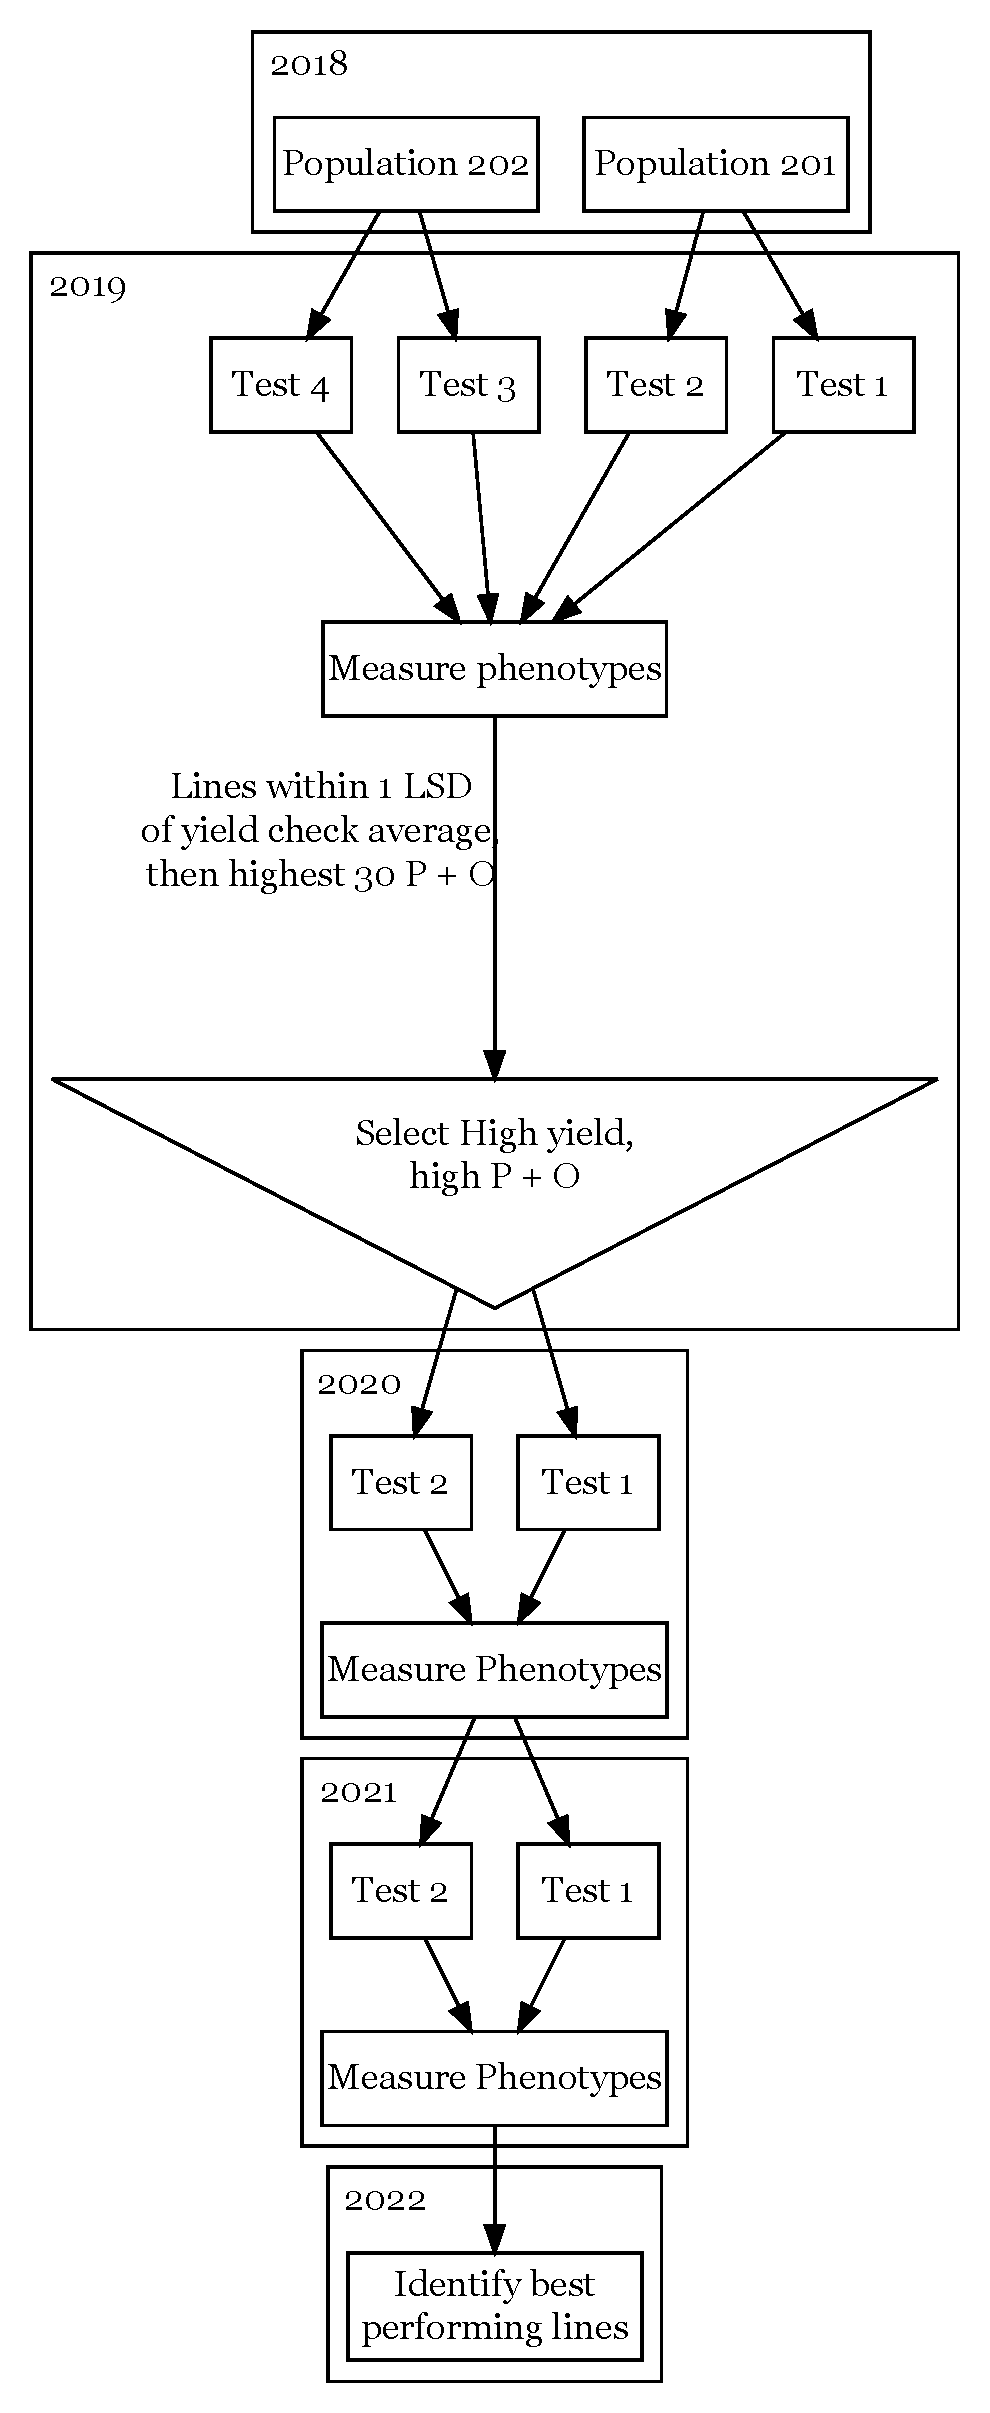
\includegraphics{C:/Users/Jay/Desktop/Documents/R/Jay_yield/exports/plots/pop_development_flowchart} \end{center}

\hypertarget{collected-data}{%
\subsection{Collected data}\label{collected-data}}

The main traits we're interested in analyzing/summarizing are yield and
the seed composition traits seed protein and oil. We do however have
data on several agronomic traits including height, maturity date, seed
weight, seed quality, and lodging. Yield was measured for all reps for
both years while seed protein and oil were measured for reps 1-2 for
both years.

\hypertarget{analysis-and-questions}{%
\subsection{Analysis and questions}\label{analysis-and-questions}}

We used a linear model to analyze the data with the formula:

\[y = \mu + GEN + ENV + GEN:ENV + REP(ENV) + \epsilon\]

Where y is the value of some phenotype, \(\mu\) is the overall mean, GEN
is the genotype effect, ENV is the environment effect, GEN:ENV is the
genotype x environment interaction effect, REP(ENV) is the effect of
replication nested within environment, and \(\epsilon\) is the
measurement error. This model was used to perform an analysis of
variance and to obtain genotype least square means.

Going back to the overall goal of the experiment, we want to identify
genotypes which have a yield comparable to or superior to that of some
existing high-yielding cultivars, and seed composition traits that are
superior to those high-yielding cultivars. The criteria by which we can
declare that a RIL has these qualities is where I have the most
questions. I've seen a few papers that used a least-significant
difference value to compare means of new cultivars to other established
cultivars and was wondering if this would be an appropriate test to use.
I have also read a fair amount of criticism for using the least
significant difference to compare means since it doesn't correct for
multiple comparisons. Because of that, I was considering using Tukeys
HSD instead, or another correction to the standard LSD test to account
for multiple comparisons. We also used multiple check cultivars within
each test, but as far as I can tell the multiple comparison statistics
are only strictly appropriate for comparing the means of one cultivar
with the means of one other, and I didn't know how appropriate it would
be to use a LSD/HSD value to compare the mean of one RIL with the
average of the checks for each test.

\end{document}
